

\tikzset{every picture/.style={line width=0.75pt}} %set default line width to 0.75pt        
\noindent
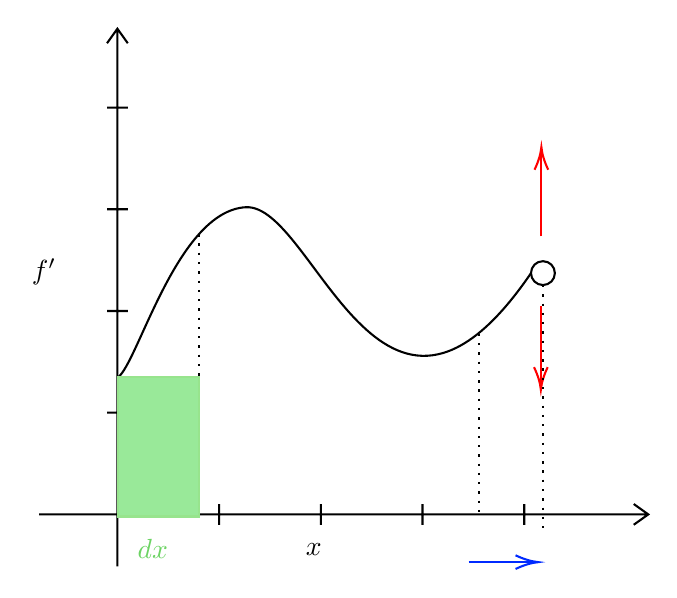
\begin{tikzpicture}[x=0.75pt,y=0.75pt,yscale=-1,xscale=1]
%uncomment if require: \path (0,300); %set diagram left start at 0, and has height of 300

%Shape: Axis 2D [id:dp40268293355011053] 
\draw  (59,251) -- (352.5,251)(96.73,17) -- (96.73,276) (345.5,246) -- (352.5,251) -- (345.5,256) (91.73,24) -- (96.73,17) -- (101.73,24) (145.73,246) -- (145.73,256)(194.73,246) -- (194.73,256)(243.73,246) -- (243.73,256)(292.73,246) -- (292.73,256)(91.73,202) -- (101.73,202)(91.73,153) -- (101.73,153)(91.73,104) -- (101.73,104)(91.73,55) -- (101.73,55) ;
\draw   ;
%Shape: Circle [id:dp27652033411617516] 
\draw   (296,134.75) .. controls (296,131.57) and (298.57,129) .. (301.75,129) .. controls (304.93,129) and (307.5,131.57) .. (307.5,134.75) .. controls (307.5,137.93) and (304.93,140.5) .. (301.75,140.5) .. controls (298.57,140.5) and (296,137.93) .. (296,134.75) -- cycle ;
%Curve Lines [id:da17858959619860293] 
\draw    (97,185) .. controls (106.79,177.66) and (125.5,105) .. (158.5,103) .. controls (191.5,101) and (223.5,241) .. (296,134.75) ;
%Straight Lines [id:da9630299033013741] 
\draw [color={rgb, 255:red, 255; green, 0; blue, 0 }  ,draw opacity=1 ]   (301,117) -- (301,76) ;
\draw [shift={(301,74)}, rotate = 450] [color={rgb, 255:red, 255; green, 0; blue, 0 }  ,draw opacity=1 ][line width=0.75]    (10.93,-3.29) .. controls (6.95,-1.4) and (3.31,-0.3) .. (0,0) .. controls (3.31,0.3) and (6.95,1.4) .. (10.93,3.29)   ;
%Straight Lines [id:da6584610678809868] 
\draw [color={rgb, 255:red, 255; green, 0; blue, 0 }  ,draw opacity=1 ]   (300.75,150.5) -- (300.75,189) ;
\draw [shift={(300.75,191)}, rotate = 270] [color={rgb, 255:red, 255; green, 0; blue, 0 }  ,draw opacity=1 ][line width=0.75]    (10.93,-3.29) .. controls (6.95,-1.4) and (3.31,-0.3) .. (0,0) .. controls (3.31,0.3) and (6.95,1.4) .. (10.93,3.29)   ;
%Straight Lines [id:da3413840183352358] 
\draw  [dash pattern={on 0.84pt off 2.51pt}]  (301.75,140.5) -- (301.75,259) ;
%Straight Lines [id:da3456990383666756] 
\draw [color={rgb, 255:red, 0; green, 42; blue, 255 }  ,draw opacity=1 ]   (266,274) -- (297.5,274) ;
\draw [shift={(299.5,274)}, rotate = 180] [color={rgb, 255:red, 0; green, 42; blue, 255 }  ,draw opacity=1 ][line width=0.75]    (10.93,-3.29) .. controls (6.95,-1.4) and (3.31,-0.3) .. (0,0) .. controls (3.31,0.3) and (6.95,1.4) .. (10.93,3.29)   ;
%Straight Lines [id:da5576696604138862] 
\draw  [dash pattern={on 0.84pt off 2.51pt}]  (271,164) -- (271,250) ;
%Straight Lines [id:da770134158979629] 
\draw  [dash pattern={on 0.84pt off 2.51pt}]  (136,116) -- (136,252) ;
%Shape: Rectangle [id:dp4648872043123744] 
\draw  [color={rgb, 255:red, 151; green, 228; blue, 141 }  ,draw opacity=1 ][fill={rgb, 255:red, 153; green, 233; blue, 153 }  ,fill opacity=1 ] (97,185) -- (136,185) -- (136,252) -- (97,252) -- cycle ;

% Text Node
\draw (54,126.4) node [anchor=north west][inner sep=0.75pt]    {$f'$};
% Text Node
\draw (186,263.4) node [anchor=north west][inner sep=0.75pt]    {$x$};
% Text Node
\draw (105,261.4) node [anchor=north west][inner sep=0.75pt]  [color={rgb, 255:red, 108; green, 211; blue, 99 }  ,opacity=1 ]  {$dx$};


\end{tikzpicture}
